
\title{A simple statistical model describing fire through its limitations}
\author{
        Douglas Kelley \\
                Centre for Ecology and Hydrology\\
	Maclean Building \\
	Crowmarsh Gifford \\
	Wallingford \\
	Oxfordshire, OX10 8BB \\
	\textbf{Email:} douglas.i.kelley@gmail.com \\
	\textbf{Web}: douglask3.github.io
%            \and
%        Yossi Gil\\
%        Department of Computer Science\\
%        Technion---Israel Institute of Technology\\
%        Technion City, Haifa 32000, \underline{Israel}
}
\date{\today}

\documentclass[12pt]{article}

\usepackage[english]{babel}
\usepackage{graphicx}
\usepackage{natbib}
\usepackage{gitinfo2}
\usepackage{amsmath}


\begin{document}
\maketitle

\begin{abstract}
LimFIRE is a simple statistical model that simulates limitations of fire. Perfect fire conditions are imagined for a location or grid cell, with full fuel coverage, no moisture, saturated igntions and no agricultural or urban fragmentation. In such conditions, 100\% of the land area burns. This is analogous to areas in Northern Australia and parts of the sahel, with areas burning more than once a year. Burnt area is reduced if the location has discontinuous fuel loads  (e.g. desert areas), has fuel to moist to burn (meg. Humid evergreen forests), a lack of ignition (shown to be an influence of inter Annual variability in some parts of the tropical vdv and Southern Australia Bradstock), or human fire suppression (e.g. cropland or urban areas).
\end{abstract}

\begin{center}
    \textbf{git info}

        git url: https://github.com/douglask3/LimFIRE

	git revision no: \gitAbbrevHash

	Last commit author: \gitAuthorName,  \gitAuthorEmail

	Branch: \gitReferences

	Revision Date: \gitAuthorIsoDate
\end{center}

\section{Introduction}
LimFIRE is a simple statistical model that simulates limitations of fire. Perfect fire conditions are imagined for a location or grid cell, with full fuel coverage, no moisture, saturated igntions and no agricultural or urban fragmentation. In such conditions, 100\% of the land area burns. This is analogous to areas in Northern Australia and parts of the sahel, with areas burning more than once a year. Burnt area is reduced if the location has discontinuous fuel loads  (e.g. desert areas), has fuel to moist to burn (meg. Humid evergreen forests), a lack of ignition (shown to be an influence of inter Annual variability in some parts of the tropical vdv and Southern Australia Bradstock), or human fire suppression (e.g. cropland or urban areas).

\paragraph{Outline}
%The remainder of this article is organized as follows.
%Section~\ref{previous work} gives account of previous work.
%Our new and exciting results are described in Section~\ref{results}.
%Finally, Section~\ref{conclusions} gives the conclusions.

\section{Methods}

\subsection{Fuel}

%\begin{equation}
%    x=\frac{1+y}{1+2z^2}
%\end{equation}

%\section{Previous work}\label{previous work}
%A much longer \LaTeXe{} example was written by Gil~\cite{Gil:02}.


\begin{figure}[!ht]
  \centering
    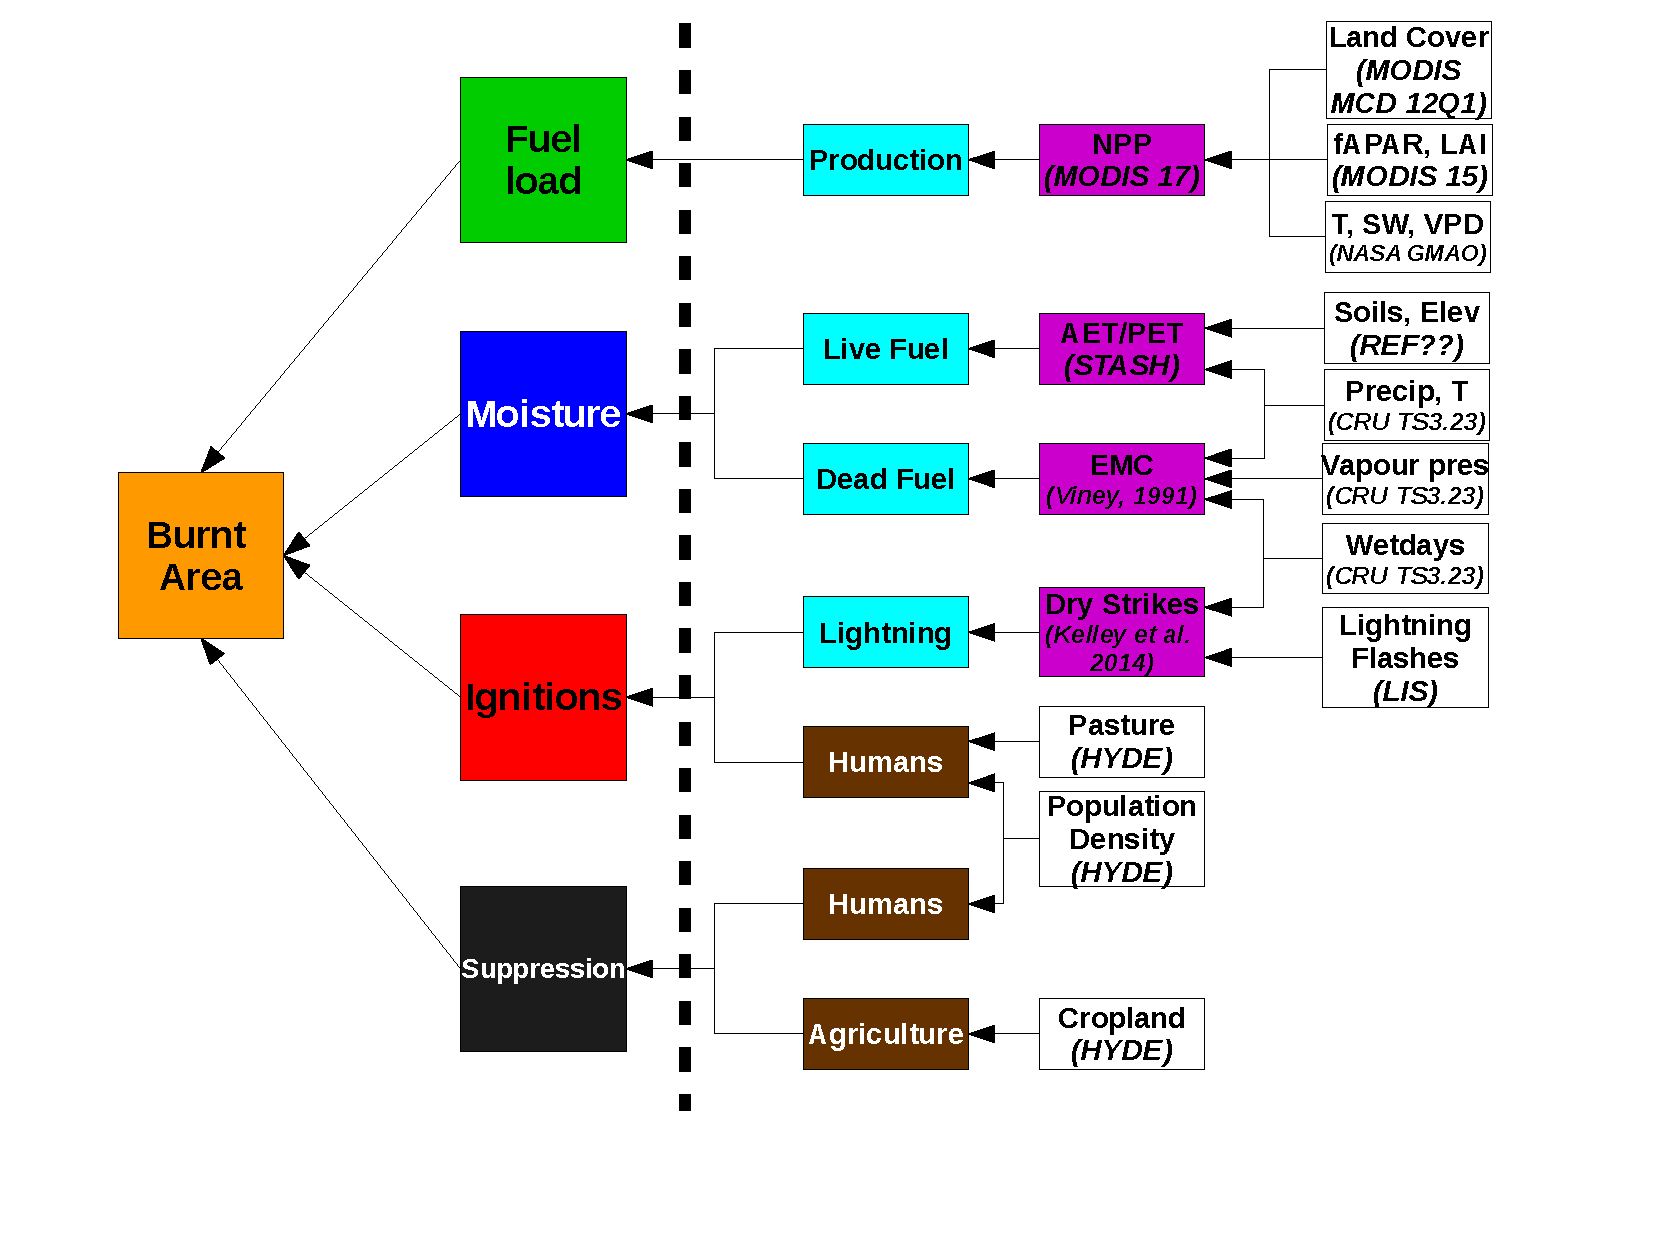
\includegraphics[width=0.67\textwidth]{Model_schematic.pdf}

  \caption{Model description.}
\end{figure}

\begin{figure}[!ht]
  \centering
    \includegraphics[width=0.67\textwidth]{../figs/gfedComparison.png}

  \caption{Bechmark comparisons against GFED4s \citep{Giglio2013}.}
\end{figure}


\begin{figure}[!ht]
  \centering
    \includegraphics[width=0.67\textwidth]{../figs/limitation_lines.png}

  \caption{Limitation covers.}
\end{figure}

\section{Results}\label{results}
In this section we describe the results.

\section{Conclusions}\label{conclusions}
We worked hard, and achieved very little.

\bibliographystyle{abbrv}
\bibliography{Model_description}

\end{document}
This is never printed
